\chapter{General Introduction}
\label{chap:introduction}

\section{General Context}
\label{sec:general-context}

Financial markets process trillions of dollars in transactions daily across equities, currencies, commodities, and digital assets. Over the past two decades, algorithmic trading has evolved from a niche practice used by quantitative hedge funds into the dominant force in global markets, now accounting for the majority of daily trading volume on major exchanges.

The core appeal is clear: algorithms process data at speeds no human can match and are immune to emotional bias. Yet building a consistently profitable system remains one of the hardest problems in applied machine learning. Markets are non-stationary --- their statistical properties shift over time. A strategy that excels during a trending bull market may fail entirely in a volatile, mean-reverting environment. This sensitivity to changing market conditions is not a minor detail; it is the central challenge of the field.

Early rule-based systems lacked adaptability. Machine learning, and reinforcement learning in particular, offered a path forward by framing trading as a sequential decision problem. More recently, large language models introduced the ability to reason over unstructured data --- news, macroeconomic commentary, sentiment --- opening a new dimension in trading research. However, existing systems that combine these approaches share a critical blind spot: none condition their decisions on an \emph{explicit}, statistically estimated representation of the current market regime shared across their reasoning and execution components, and few test whether such conditioning actually helps against a proper noise control. This gap defines the motivation for MARTA.

\section{Host Organization}
\label{sec:host-organization}

\subsection{Presentation of Coral-io}
\label{subsec:coral-io-presentation}

Coral-io (registered as Coralio Software, Les Berges du Lac, Tunis) is a technology consulting firm specializing in digital transformation and IT solutions across multiple industries. The company provides comprehensive services that bridge technical expertise with business objectives, helping clients navigate complex technological challenges. Its activity spans five main areas:

\begin{itemize}
    \item \textbf{DevOps Services}: CI/CD pipeline implementation, Infrastructure as Code, containerization and orchestration (Docker, Kubernetes), and test automation.
    \item \textbf{Application Performance Management (APM)}: full-stack observability, real-time monitoring, and bottleneck diagnosis for production software.
    \item \textbf{Third-Party Solution Integration}: as a Micro Focus (OpenText) partner, Coral-io delivers IT Operations Management (ITOM) integration and legacy system modernization.
    \item \textbf{Research \& Development}: proof-of-concept development and emerging-technology adoption, sitting at the intersection of technical expertise and applied innovation.
    \item \textbf{Finance and Insurance Consulting}: FinTech implementation, regulatory compliance, and digital transformation for financial services clients.
\end{itemize}

MARTA was carried out within the R\&D and Finance/Insurance Consulting scope of the company's activity, combining applied AI research with a financial-markets use case.

\subsection{Internship Framework}
\label{subsec:internship-framework}

Unlike a project built around a pre-defined internal need, this final-year project was conducted under a self-directed research framework: Coral-io granted full autonomy in selecting the subject and technical direction of the work.

Within this framework, technical guidance was provided collaboratively by Ms. Oumaima Aounallah and the wider Coral-io team, consulted on an as-needed basis for architectural decisions, tooling questions, and periodic progress reviews rather than through prescriptive task assignment. Academic supervision was provided by Saoussen Lakhdhar at ESPRIT.

This structure placed a greater share of responsibility for scoping, planning, and technical decision-making than is typical of a company-assigned project --- a distinction elaborated further in Section~\ref{sec:methodology-planning}.

\section{Problem Statement}
\label{sec:problem-statement}

\subsection{Limitations of Existing Approaches}
\label{subsec:limitations-existing}

Three broad families of automated trading systems exist today, each with a distinct blind spot relevant to MARTA.

\textbf{Rule-based and classical statistical strategies} (moving-average crossovers, mean-reversion bands, momentum filters) are transparent and computationally cheap, but their parameters are fixed at design time. When the market regime shifts --- from trending to ranging, from low to high volatility --- these fixed parameters no longer match the underlying data-generating process, and performance degrades until the strategy is manually re-tuned.

\textbf{Pure reinforcement learning agents} address this rigidity by learning a policy directly from historical price action, allowing some adaptation to changing dynamics. However, standard RL formulations treat the market as a single, undifferentiated environment: the agent is not explicitly told which regime it is currently operating in, and must infer this implicitly through its state representation. In practice, this means the policy tends to average its behavior across regimes rather than specializing for each one, and offers no human-interpretable explanation for why a given action was chosen.

\textbf{LLM-based trading agents}, a more recent development, exploit large language models' ability to reason over unstructured text --- news headlines, macroeconomic reports, analyst commentary --- to produce qualitative market assessments. This adds a reasoning layer absent from purely numerical approaches, and can in principle justify its decisions in natural language. However, existing systems in this category typically condition the LLM's reasoning only on recent price statistics or raw text, without any structured, explicit signal describing the broader statistical regime the market is currently in.

\subsection{The Core Gap}
\label{subsec:core-gap}

Across all three families, no system combines (i) an explicit, probabilistic regime signal estimated from data, (ii) multi-perspective reasoning conditioned on that same signal, and (iii) an execution layer able to adapt its risk behavior to it --- and, just as importantly, prior work rarely tests whether regime conditioning helps by comparing it against a matched noise control rather than against a weak baseline. Regime is either ignored entirely, treated as a hidden variable an RL agent must discover implicitly, or left to ad hoc heuristics (e.g., a simple volatility threshold) rather than estimated from data.

\subsection{Formal Problem Statement}
\label{subsec:formal-problem}

Given a multi-asset time series of market data, the problem addressed by this work is twofold:

\begin{enumerate}
    \item \textbf{Regime representation}: derive an explicit, probabilistic representation of market regime from data, with interpretable transition dynamics, without relying on hand-labeled regimes.
    \item \textbf{Regime-conditioned decision making}: use this representation to condition both a multi-perspective reasoning process and a downstream execution policy, such that trading behavior adapts to the identified regime rather than applying a single fixed strategy across all market conditions.
\end{enumerate}

Success is measured not only by trading performance (risk-adjusted returns, drawdown) but by whether regime conditioning demonstrably improves outcomes relative to regime-agnostic baselines --- the central empirical question this report answers in Chapter~\ref{chap:results}.

\section{Proposed Solution}
\label{sec:proposed-solution}

MARTA addresses this gap through a five-layer pipeline, each layer directly targeting one part of the problem statement above.

\begin{enumerate}
    \item \textbf{Feature Engineering}: a set of engineered technical and statistical indicators (volatility, momentum, trend, and higher-moment statistics) is computed per asset from hourly multi-asset crypto data (BTC, ETH, BNB, LTC, XRP), providing the market-state representation regime detection operates on directly, without requiring hand-labeled regimes. A learned alternative (a Temporal Fusion Transformer encoder trained with an InfoNCE contrastive objective) and an initial mixed crypto/traditional-finance panel were both evaluated and replaced, for reasons given in Chapter~\ref{chap:methodology}.
    \item \textbf{Regime Detection}: a Gaussian Hidden Markov Model is fitted directly on the engineered feature space, discretizing market state into a small number of interpretable, statistically distinct regimes with associated transition dynamics.
    \item \textbf{Multi-Agent Deliberation}: five specialist agents --- three LLM agents forming directional views (macro, technical, sentiment), a contrarian agent whose opposing direction is fixed in code, and a non-LLM GARCH risk agent --- feed a Fund Manager agent that aggregates them deterministically into a regime-aware, risk-capped recommendation with a natural-language rationale, rather than a black-box signal.
    \item \textbf{RL Execution Agent}: a PPO-trained agent designed to translate market state, regime, and agent consensus into position sizing. In the evaluated checkpoints it operates on engineered features and is trained and evaluated as a separate component that does not consume the debate output (Section~\ref{subsec:agent-rl-disconnect}).
    \item \textbf{Monitoring Dashboard}: a Next.js interface exposes regime detection, agent reasoning, and execution decisions in real time, making the system's behavior auditable rather than opaque.
\end{enumerate}

This layered design directly mirrors the two-part problem statement: layers 1--2 address the regime representation problem, and layers 3--4 solve the regime-conditioned decision making problem. Layer 5 is a supporting component providing interpretability rather than a decision-making stage in its own right. The empirical contribution of regime-awareness across layers 1--4 is evaluated through dedicated ablation studies, presented in Chapter~\ref{chap:results}.

\begin{figure}[!htbp]
    \centering
    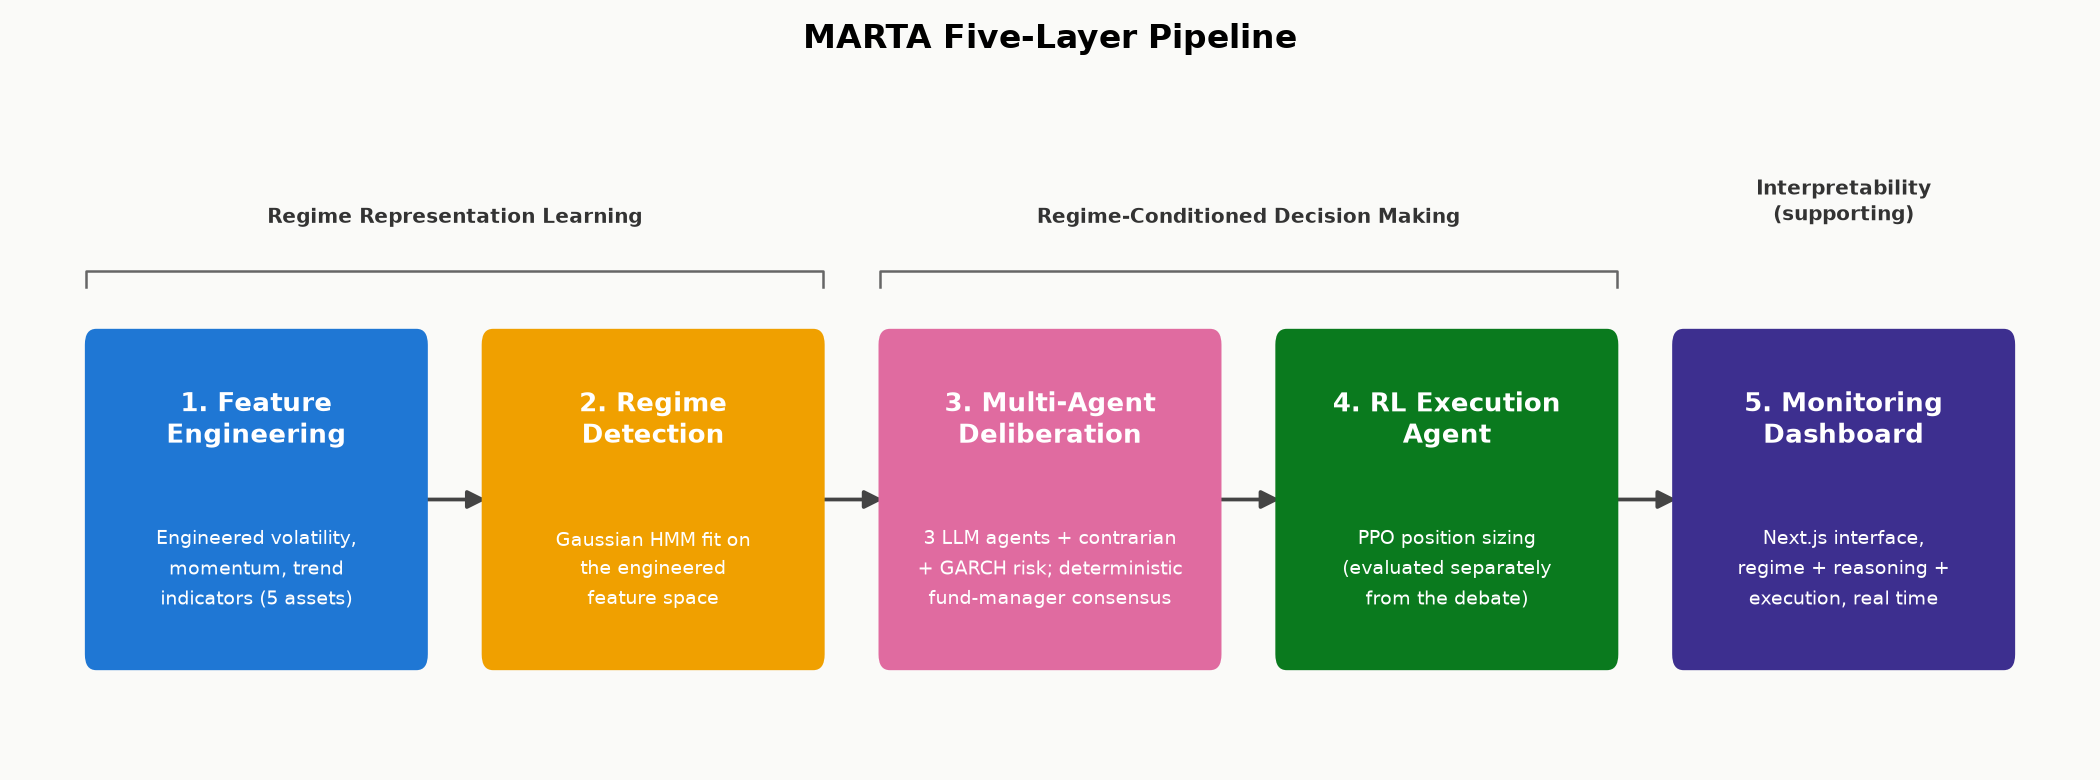
\includegraphics[width=\textwidth]{images/pipeline_diagram.png}
    \caption{MARTA's five-layer pipeline, grouped according to the two-part problem statement of Section~\ref{subsec:formal-problem}. Each layer is detailed in Chapter~\ref{chap:methodology}.}
    \label{fig:pipeline}
\end{figure}

\section{Project Objectives and Scope}
\label{sec:objectives-scope}

\subsection{Objectives}
\label{subsec:objectives}

The project pursues four concrete objectives, each corresponding to a layer of the proposed solution:

\begin{enumerate}
    \item \textbf{Build a meaningful regime representation}: engineer a multi-asset hourly feature set (volatility, momentum, trend, and higher-moment statistics) that captures structure relevant to near-term market dynamics, validated through downstream regime separability once clustered by the HMM.
    \item \textbf{Discover interpretable, statistically distinct regimes}: fit a Gaussian HMM directly over the engineered feature space and verify that the resulting regimes are stable, distinguishable, and align with intuitive market conditions (e.g., trending vs.\ ranging, high vs.\ low volatility) upon inspection.
    \item \textbf{Build a regime-aware multi-agent reasoning layer}: design and implement a multi-agent LLM deliberation system whose recommendations are conditioned on detected regime, and evaluate whether this conditioning improves recommendation quality over a regime-agnostic baseline.
    \item \textbf{Train an adaptive execution policy}: implement a PPO-based execution agent that produces position-sizing decisions, and evaluate --- via ablation --- whether regime-awareness measurably improves risk-adjusted trading performance relative to an equivalent regime-agnostic system.
\end{enumerate}

A secondary, supporting objective is to expose the full pipeline through a monitoring dashboard, so that regime detection, agent reasoning, and execution decisions remain auditable rather than opaque --- a property largely absent from prior work in this space (Section~\ref{subsec:limitations-existing}).

\subsection{Scope}
\label{subsec:scope}

\textbf{In scope:}
\begin{itemize}
    \item Five crypto assets: BTC/USDT, ETH/USDT, BNB/USDT, LTC/USDT, XRP/USDT, at hourly resolution, 2018--2025. An initial four-asset panel spanning crypto and traditional-finance instruments (BTC/USD, ETH/USD, EUR/USD, XAU/USD) was revised to this crypto-only panel after a data-quality defect specific to the traditional-finance instruments was diagnosed (Chapter~\ref{chap:methodology}).
    \item Design, training, and evaluation of all five architectural layers described in Section~\ref{sec:proposed-solution}.
    \item Backtesting and ablation studies quantifying the contribution of regime-awareness specifically.
    \item A functional monitoring dashboard for the full pipeline.
\end{itemize}

\textbf{Out of scope:}
\begin{itemize}
    \item Live deployment with real capital; the system is evaluated via backtesting and paper-trading simulation only.
    \item Assets or timeframes beyond the five instruments and hourly resolution listed above.
    \item Regulatory, compliance, or brokerage-integration work required for production trading.
    \item Optimization of LLM inference cost/latency for high-frequency use cases; the multi-agent layer operates at hourly decision frequency, not tick-level.
\end{itemize}

This scope reflects the project's nature as an applied research contribution demonstrating the value of regime-awareness, rather than a production-ready trading product.

\section{Requirements Specification}
\label{sec:requirements-specification}

The objectives of Section~\ref{sec:objectives-scope} state \emph{what} the project set out to demonstrate; this section restates the same commitments as concrete, individually checkable requirements, in the functional/non-functional form expected of an engineering deliverable, and points each one to the chapter and section where it is actually discharged and evidenced, rather than only asserted here.

\subsection{Functional Requirements}
\label{subsec:functional-requirements}

\begin{itemize}
    \item \textbf{FR1 --- Regime representation.} The system shall derive a market-state representation from multi-asset OHLCV data without relying on hand-labeled regimes. \emph{Discharged by:} Section~\ref{sec:data-feature-engineering} (feature engineering) and Section~\ref{sec:regime-encoder-methodology} (the superseded learned-encoder variant).
    \item \textbf{FR2 --- Regime detection.} The system shall discretize market state into a small number of statistically distinct regimes with explicit transition dynamics, and that distinctness shall be verified, not assumed. \emph{Discharged by:} Section~\ref{sec:regime-detection-methodology}; verified in Section~\ref{subsec:regime-results-preview} (volatility distinctness, $p\approx0$ across every configuration tested).
    \item \textbf{FR3 --- Regime-conditioned multi-agent reasoning.} The system shall produce a directional trading recommendation from multiple specialized perspectives, each explicitly conditioned on the detected regime rather than reasoning over price alone. \emph{Discharged by:} Section~\ref{sec:multi-agent-methodology}; verified in Section~\ref{subsec:agent-validation-battery} (the null-regime test, confirming regime context is not silently discarded).
    \item \textbf{FR4 --- Learned execution policy.} The system shall translate agent consensus and portfolio state into position-sizing decisions via a trained policy rather than a fixed rule. \emph{Discharged by:} Section~\ref{sec:rl-execution-methodology}.
    \item \textbf{FR5 --- Live monitoring.} The system shall expose regime detection, agent reasoning, and execution decisions through a real-time interface. \emph{Discharged by:} Section~\ref{sec:dashboard-methodology}.
    \item \textbf{FR6 --- Decision auditability.} Every displayed decision (action, position size, conviction) shall be traceable to the specific inputs --- regime, consensus, risk limits --- that produced it, and every quantity shown alongside a decision shall originate from the same evaluation run as that decision. \emph{Discharged by:} Section~\ref{subsec:dashboard-auditability}.
\end{itemize}

\subsection{Non-Functional Requirements}
\label{subsec:non-functional-requirements}

\begin{itemize}
    \item \textbf{NFR1 --- Evaluation determinism.} Repeated evaluation of an identical checkpoint under an identical configuration shall return bit-identical metrics, so that a reported result is attributable to the checkpoint and configuration rather than to run-to-run noise. \emph{Discharged by:} Section~\ref{subsec:rl-determinism}.
    \item \textbf{NFR2 --- Data integrity / no leakage.} No training, model-selection, or hyperparameter decision shall read data from the test split; this boundary shall be asserted in code, not only documented. \emph{Discharged by:} Section~\ref{subsec:train-val-test-split}.
    \item \textbf{NFR3 --- Statistical rigor.} Every headline performance comparison shall be reported with a significance test or an explicit noise control, not as an isolated point estimate. \emph{Discharged by:} Section~\ref{subsec:eval-bootstrap}; applied throughout Chapter~\ref{chap:results}.
    \item \textbf{NFR4 --- Modularity and maintainability.} The five architectural layers shall be independently revisable --- a change to one layer (e.g.\ the regime detector's asset panel) shall not require redesigning the layers downstream of it. \emph{Discharged by:} the layered design of Section~\ref{sec:proposed-solution}; exercised in practice when the asset-panel revision of Section~\ref{subsec:regime-asset-panel-revision} and the encoder's retirement (Section~\ref{subsec:encoder-refinement}) were both absorbed without a redesign of the multi-agent or dashboard layers.
    \item \textbf{NFR5 --- Operational responsiveness.} The live system shall produce one regime/consensus/execution decision per asset per hour, matching the pipeline's native data resolution. \emph{Discharged by:} Section~\ref{subsec:dashboard-architecture} (the APScheduler-driven hourly signal tick).
\end{itemize}

\section{Project Methodology and Work Planning}
\label{sec:methodology-planning}

Given the exploratory, research-oriented nature of MARTA, a rigid upfront specification was not appropriate: each architectural layer's design depended on empirical results from the layer built before it (e.g., the number and structure of latent regimes discovered by the HMM directly shaped how agent prompts were engineered). The project therefore followed an \textbf{iterative, layer-by-layer methodology}, where each phase produced a working, evaluable component before the next was started, rather than a big-bang integration at the end.

\subsection{Choice of Methodology: CRISP-DM over Sprint-Based Agile}
\label{subsec:methodology-comparison}

Sprint-based Agile frameworks (Scrum, Kanban) were considered and set aside. Both assume a backlog of comparatively independent, estimable units of work that can be committed to a fixed-length iteration; MARTA's work plan did not have that shape. The content of a given phase's deliverable --- how many regimes the HMM would discover, whether the learned encoder would outperform raw features, which architectural lever (if any) would close the RL layer's gap to buy-and-hold --- was not knowable until the previous phase's empirical results were in hand, so committing a sprint's scope in advance would have meant committing to work that later evidence twice required reopening (Section~\ref{subsec:regime-asset-panel-revision}'s panel revision and Section~\ref{subsec:encoder-refinement}'s encoder retirement, both triggered by evaluation outcomes rather than schedule). CRISP-DM was adopted instead specifically because its Evaluation phase is a first-class, named step that can route back to Data Preparation or Modeling, giving this evidence-driven revision pattern an explicit place in the methodology rather than treating every such revision as an exception to a Scrum backlog planned before the evidence existed.

\subsection{Development Methodology: CRISP-DM}
\label{subsec:crispdm-methodology}

MARTA's process follows CRISP-DM (Cross-Industry Standard Process for Data Mining) \cite{crispdm2000}, which organizes a data-mining project into six canonical phases: Business Understanding, Data Understanding, Data Preparation, Modeling, Evaluation, and Deployment. Table~\ref{tab:crispdm-mapping} maps each phase to the sections of this report that cover it.

CRISP-DM's defining property is that it is not a one-way pipeline: it explicitly allows evaluation in one phase to send the project back to an earlier one, and MARTA's own revision history is a direct instance of this rather than a deviation from a plan. Three examples recur throughout Chapter~\ref{chap:methodology}: evaluating the regime encoder against a raw-feature baseline (Evaluation) found it underperforming and sent the design back to Modeling, where the HMM was refit directly on engineered features instead (Section~\ref{subsec:encoder-refinement}); evaluating the resulting model against the original four-asset panel (Evaluation) found it had collapsed onto asset identity rather than market regime, sending the project back to Data Preparation to redefine the asset panel itself (Section~\ref{subsec:regime-asset-panel-revision}); and evaluating the RL execution layer's ablation (Evaluation) found no configuration beat buy-and-hold, changing the Deployment phase's default signal source accordingly (Section~\ref{subsec:rl-final-decision}). Table~\ref{tab:phases}'s nine work-plan phases are this same six-phase cycle instantiated concretely for MARTA, several of them spanning more than one CRISP-DM phase where a revision folded two stages back together.

\begin{table}[H]
\centering
\small
\caption{CRISP-DM phases}
\label{tab:crispdm-mapping}
\begin{tabular}{|l|p{9.5cm}|}
\hline
\textbf{CRISP-DM Phase} & \textbf{Report Section(s)} \\
\hline
Business Understanding & Section~\ref{sec:problem-statement} (Problem Statement), Section~\ref{sec:proposed-solution} (Proposed Solution), Section~\ref{sec:objectives-scope} (Objectives and Scope), Section~\ref{sec:requirements-specification} (Requirements Specification) \\
\hline
Data Understanding & Section~\ref{subsec:data-sources} (Data Sources and Coverage); Section~\ref{subsec:regime-asset-panel-revision} (Asset Panel Revision) \\
\hline
Data Preparation & Section~\ref{subsec:pipeline-stages} (Pipeline Stages), Section~\ref{subsec:train-val-test-split} (Train/Validation/Test Split) \\
\hline
Modeling & Section~\ref{sec:regime-encoder-methodology} (Regime Encoder), Section~\ref{sec:regime-detection-methodology} (Regime Detection), Section~\ref{sec:multi-agent-methodology} (Multi-Agent Deliberation), Section~\ref{sec:rl-execution-methodology} (RL Execution Agent) \\
\hline
Evaluation & Section~\ref{sec:evaluation-methodology-full} (Evaluation Methodology), Chapter~\ref{chap:results} (Results) \\
\hline
Deployment & Section~\ref{sec:dashboard-methodology} (Dashboard and Live System) \\
\hline
\end{tabular}
\normalsize
\end{table}

Chapter~\ref{chap:methodology}'s section order follows the same Data $\to$ Modeling $\to$ Evaluation $\to$ Deployment sequence.

\subsection{Development Phases}
\label{subsec:development-phases}

The work was organized into nine phases, summarized in Table~\ref{tab:phases} and Figure~\ref{fig:gantt}. The first five ran sequentially: literature review and architecture design, then one phase per architectural layer through the multi-agent system, each producing a working, evaluable component before the next began. The final four phases (RL execution, dashboard/live integration, encoder diagnostics, and the raw-feature pivot) overlapped rather than running strictly in sequence --- a genuine reflection of the project's last two months, during which RL training, dashboard development, and a systematic audit of the encoder were pursued concurrently, converging in the decision to drop the learned encoder in favor of engineered features (Chapter~\ref{chap:methodology}).

\begin{table}[H]
\centering
\small
\caption{MARTA development phases}
\label{tab:phases}
\begin{tabular}{|p{3.6cm}|p{4.4cm}|p{2.5cm}|p{2.6cm}|}
\hline
\textbf{Phase} & \textbf{Deliverable} & \textbf{Duration \& dates} & \textbf{CRISP-DM Phase(s)} \\
\hline
1. Literature Review \& Architecture Design & State-of-the-art survey, 5-layer design & 8 wk (Mar 16 -- May 10) & Business Understanding \\
\hline
2. Data Pipeline \& Feature Engineering & Cleaned multi-asset hourly dataset (2018--2025) & 2 wk (May 11 -- May 24) & Data Preparation \\
\hline
3. Regime Encoder (TFT + InfoNCE) --- v1 & Trained TFT + InfoNCE encoder (later superseded, Ch.~\ref{chap:methodology}) & 3 wk (May 25 -- Jun 14) & Modeling \\
\hline
4. Regime Detection (HMM) & Gaussian HMM over encoder embeddings (later refit on raw features, Ch.~\ref{chap:methodology}) & 2 wk (Jun 15 -- Jun 28) & Modeling \\
\hline
5. Multi-Agent System & Multi-agent LLM debate pipeline & 3 wk (Jun 29 -- Jul 19) & Modeling \\
\hline
6. RL Execution Agent \& Evaluation Fixes & PPO supervisor trained on agent outputs; eval-determinism and reward-scaling fixes & 6 wk (Jul 20 -- Aug 30) & Modeling, Evaluation \\
\hline
7. Dashboard \& Live Integration & Next.js dashboard, live data bridges, paper-trading execution & 6 wk (Jul 27 -- Sep 6) & Deployment \\
\hline
8. Encoder Diagnostic \& Rejected Retrains & Systematic audit of encoder retrain variants; none promoted (Ch.~\ref{chap:methodology}) & 3 wk (Aug 10 -- Aug 30) & Evaluation \\
\hline
9. Raw-Feature Pivot \& Crypto5 Migration & Encoder retired in favor of engineered features; crypto-only 5-asset panel adopted & 3 wk (Aug 27 -- Sep 16) & Data Understanding, Data Preparation, Modeling \\
\hline
\end{tabular}
\normalsize
\end{table}

\begin{figure}[!htbp]
    \centering
    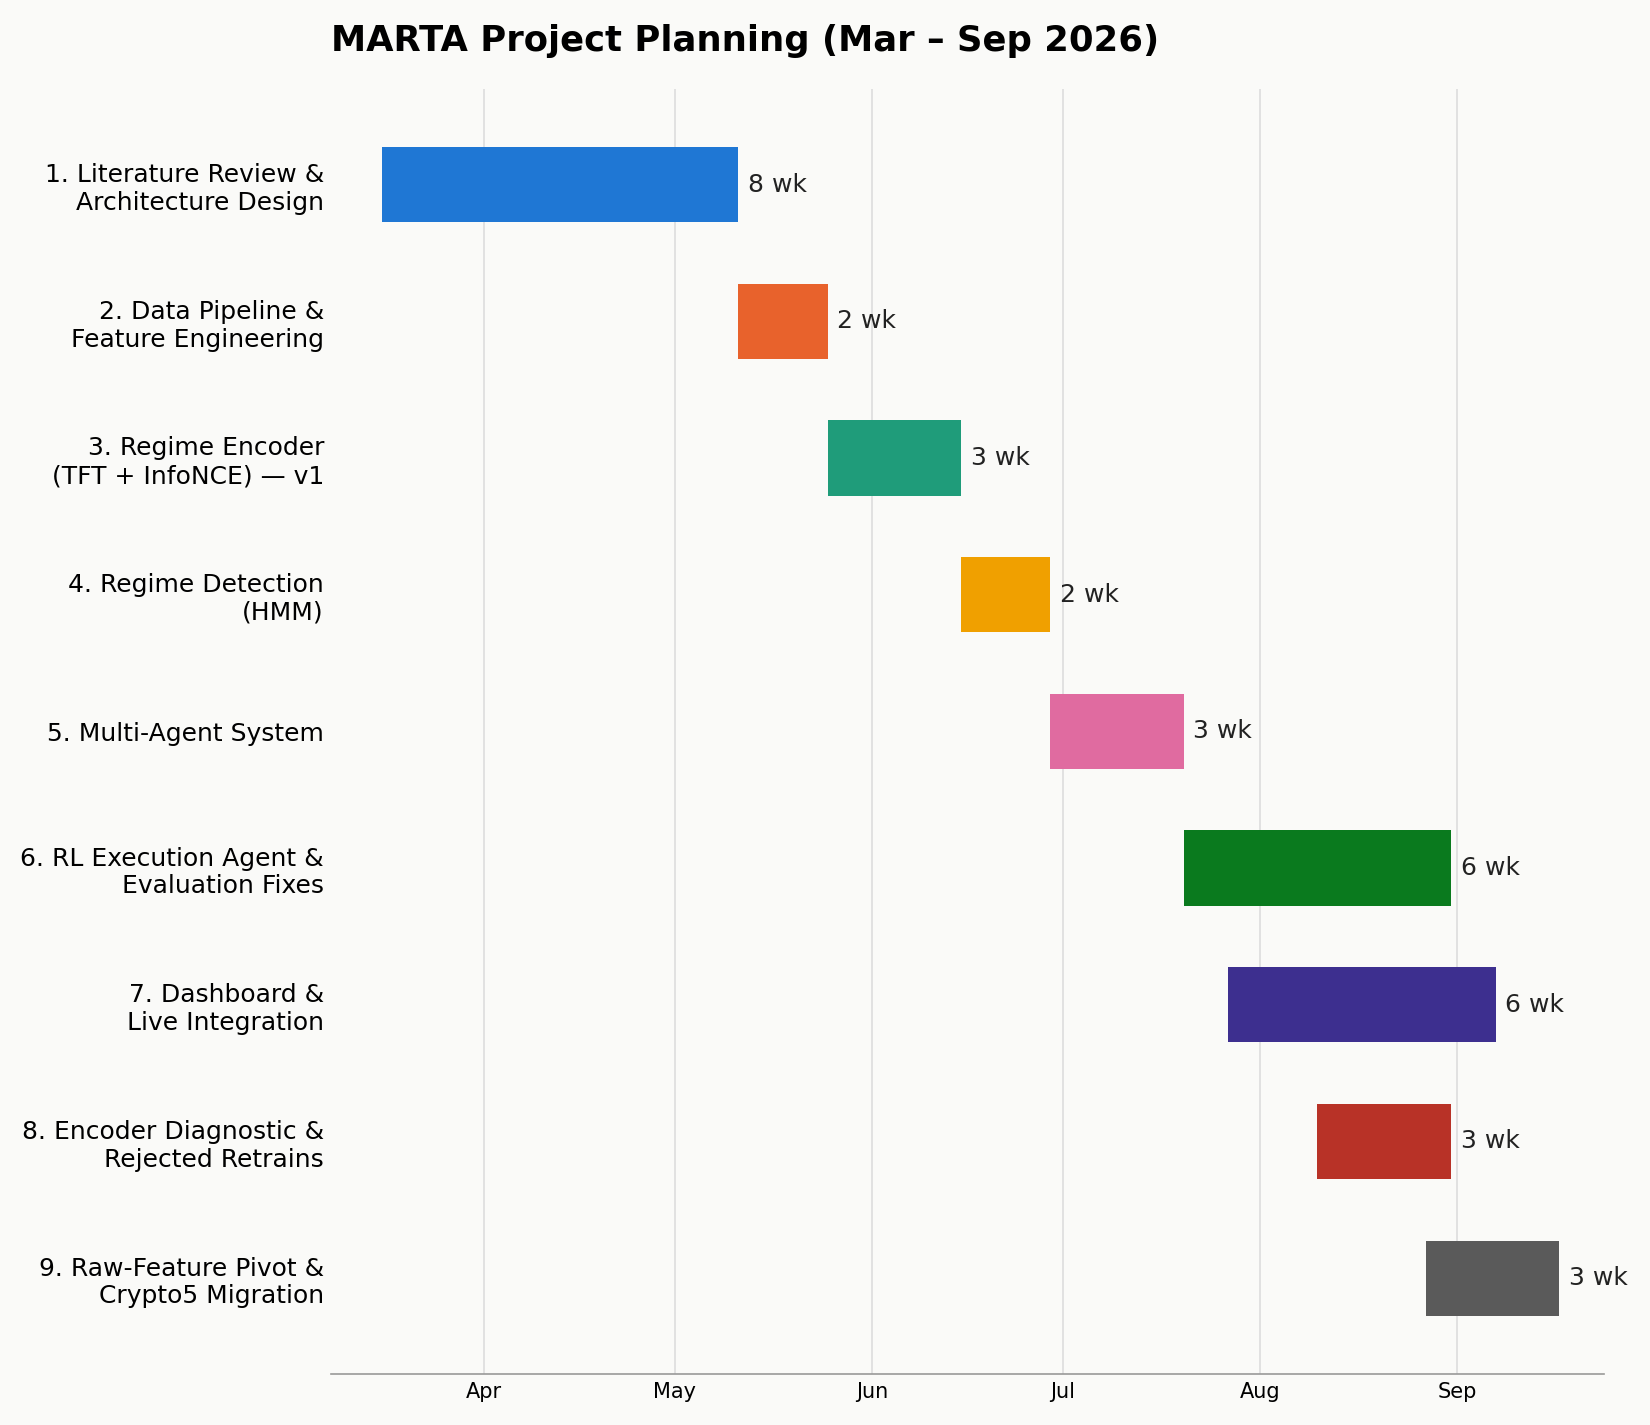
\includegraphics[width=0.85\textwidth]{images/gantt_chart.png}
    \caption{Project planning Gantt chart}
    \label{fig:gantt}
\end{figure}

\subsection{Rationale for the Approach}
\label{subsec:methodology-rationale}

This phase-by-phase structure offered two advantages over a monolithic design-then-build approach. First, it allowed early validation of the encoder and regime detection stages in isolation --- verifying, for instance, that discovered regimes were interpretable and stable before committing to an agent architecture built on top of them. Second, it kept technical risk contained: had the HMM failed to produce meaningful regime clusters, the multi-agent and RL layers could have been redesigned without discarding the data pipeline or encoder work. The overlap in phases 6--9 is itself part of that story: it was the concurrent pressure of RL evaluation work and a systematic encoder audit --- not a planned step --- that surfaced the case for the raw-feature pivot.

The sections of Chapter~\ref{chap:methodology} broadly follow this same progression; the phase 8--9 findings are folded into the discussion of the layers they ultimately affected (the Regime Encoder and Regime Detection sections) rather than given standalone sections of their own.